\documentclass[11pt,letterpaper]{article}
\usepackage[breaklinks=true,bookmarks=false]{hyperref}
\usepackage[margin=1in]{geometry}
\usepackage{amsfonts}
\usepackage{amsmath}
\usepackage{amssymb}
\usepackage{amsthm}
\usepackage{graphicx}
\usepackage{enumerate}
\usepackage{listings}
%\usepackage{subfig}
\usepackage{subfiles} % Best loaded last in the preamble
\usepackage{xcolor}
%
%
%
%\usepackage[utf8x]{inputenc}
%\usepackage{graphicx}
%\usepackage{empheq}
\usepackage{tcolorbox}
%\usepackage{bbm}	
%\usepackage{tikz}
\usepackage{biblatex}
\addbibresource{references.bib}
\begin{document}

\title{
         Exact method and Genetic algorithm for the symmetric
Travelling Salesperson Problem\\
{\normalsize in partial fulfillment for the "Methods and Models for Combinatorial Optimization" course unit}\\  
        \textsc{\normalsize Università degli Studi di Padova\\ Dipartimento di Matematica "Tullio Levi-Civita"\\ Master's Degree in Computer Science}\\
        }

\author{Luca Veronese\\
mat. 2089404\\
{\tt\small luca.veronese.5@studenti.unipd.it}
}
\clearpage
\maketitle


\subfile{section/ex01}
\subfile{section/ex02}
\section{Tests and performance}
To evaluate the performance of the algorithm, tests were conducted on a machine running Fedora Linux 40. The hardware specifications include an AMD Ryzen 5 7640U (6-core, 12-thread) processor and 32GB of DDR5 RAM (5600 MHz, dual channel).

Wall-clock time and CPU time for the exact and metaheuristic solution were measured using \texttt{/usr/bin/time}.
\subsection{Random Instance Generation}

To generate problem instances initially a standard distribution was utilized, resulting in the formation of dense clusters that are spatially separated from one another. 

To introduce additional variation and achieve a more realistic distribution, a uniform distribution was incorporated. This addition populates the remaining space with less dense points, leading to a structure that loosely resembles distinct components (clusters) connected by a sparse network of points; hopefully similar to a printed circuit layout.
\begin{figure}[h]
    \centering
    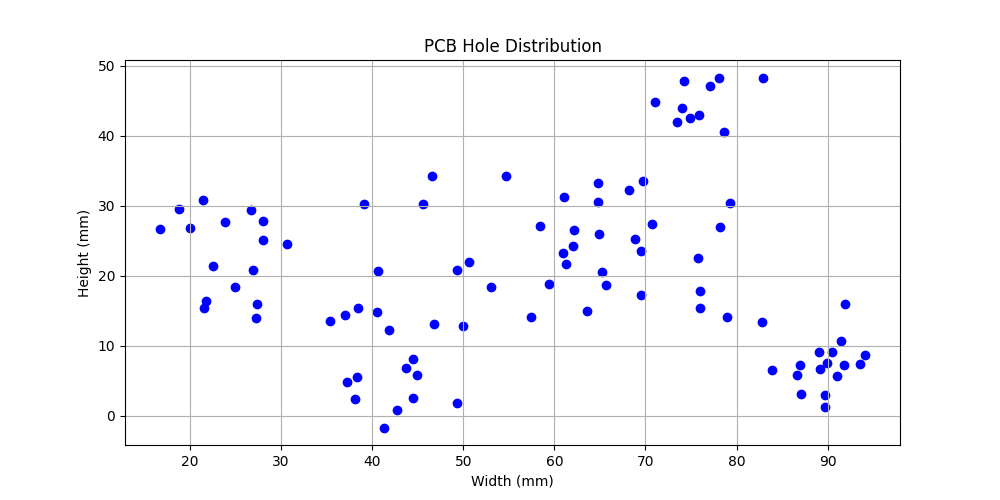
\includegraphics[width=0.8\linewidth]{../part1/inst_generator/random94.png}
    \caption{Random instance with 94 holes}
    \label{fig:random94}
\end{figure}


\section{Discussion}
The exact method was run until the optimal solution was obtained (with possible tolerance) for instances with fewer than 100 nodes. The computational complexity appears to be highly non-linear: the solver takes approximately 10 seconds to solve a 64-node instance and 80 seconds for a 94-node instance.


The genetic algorithm is effective in improving the initial population only when this population is highly unfit initially.

In facts, the presence of even a single Nearest Neighbor solution in an otherwise random initial population creates a local optimum that not a single of our genetic algorithms can overcome, causing our algorithm to output the initial solution.

In contrast, initializing the population with 10\% Farthest Insertion solutions and 90\% random permutations allows the algorithm to effectively explore and improve upon the initial solutions, never reaching the quality of a solution generated with nearest neighbor anyway.




%% \section{Bibliography}
\printbibliography
\end{document}
